La hidroeléctrica Zeus debe transferir desde su represa de agua, ubicada en el nodo 1 de la figura, hacia los generadores, ubicados en el nodo 6 de la figura.

%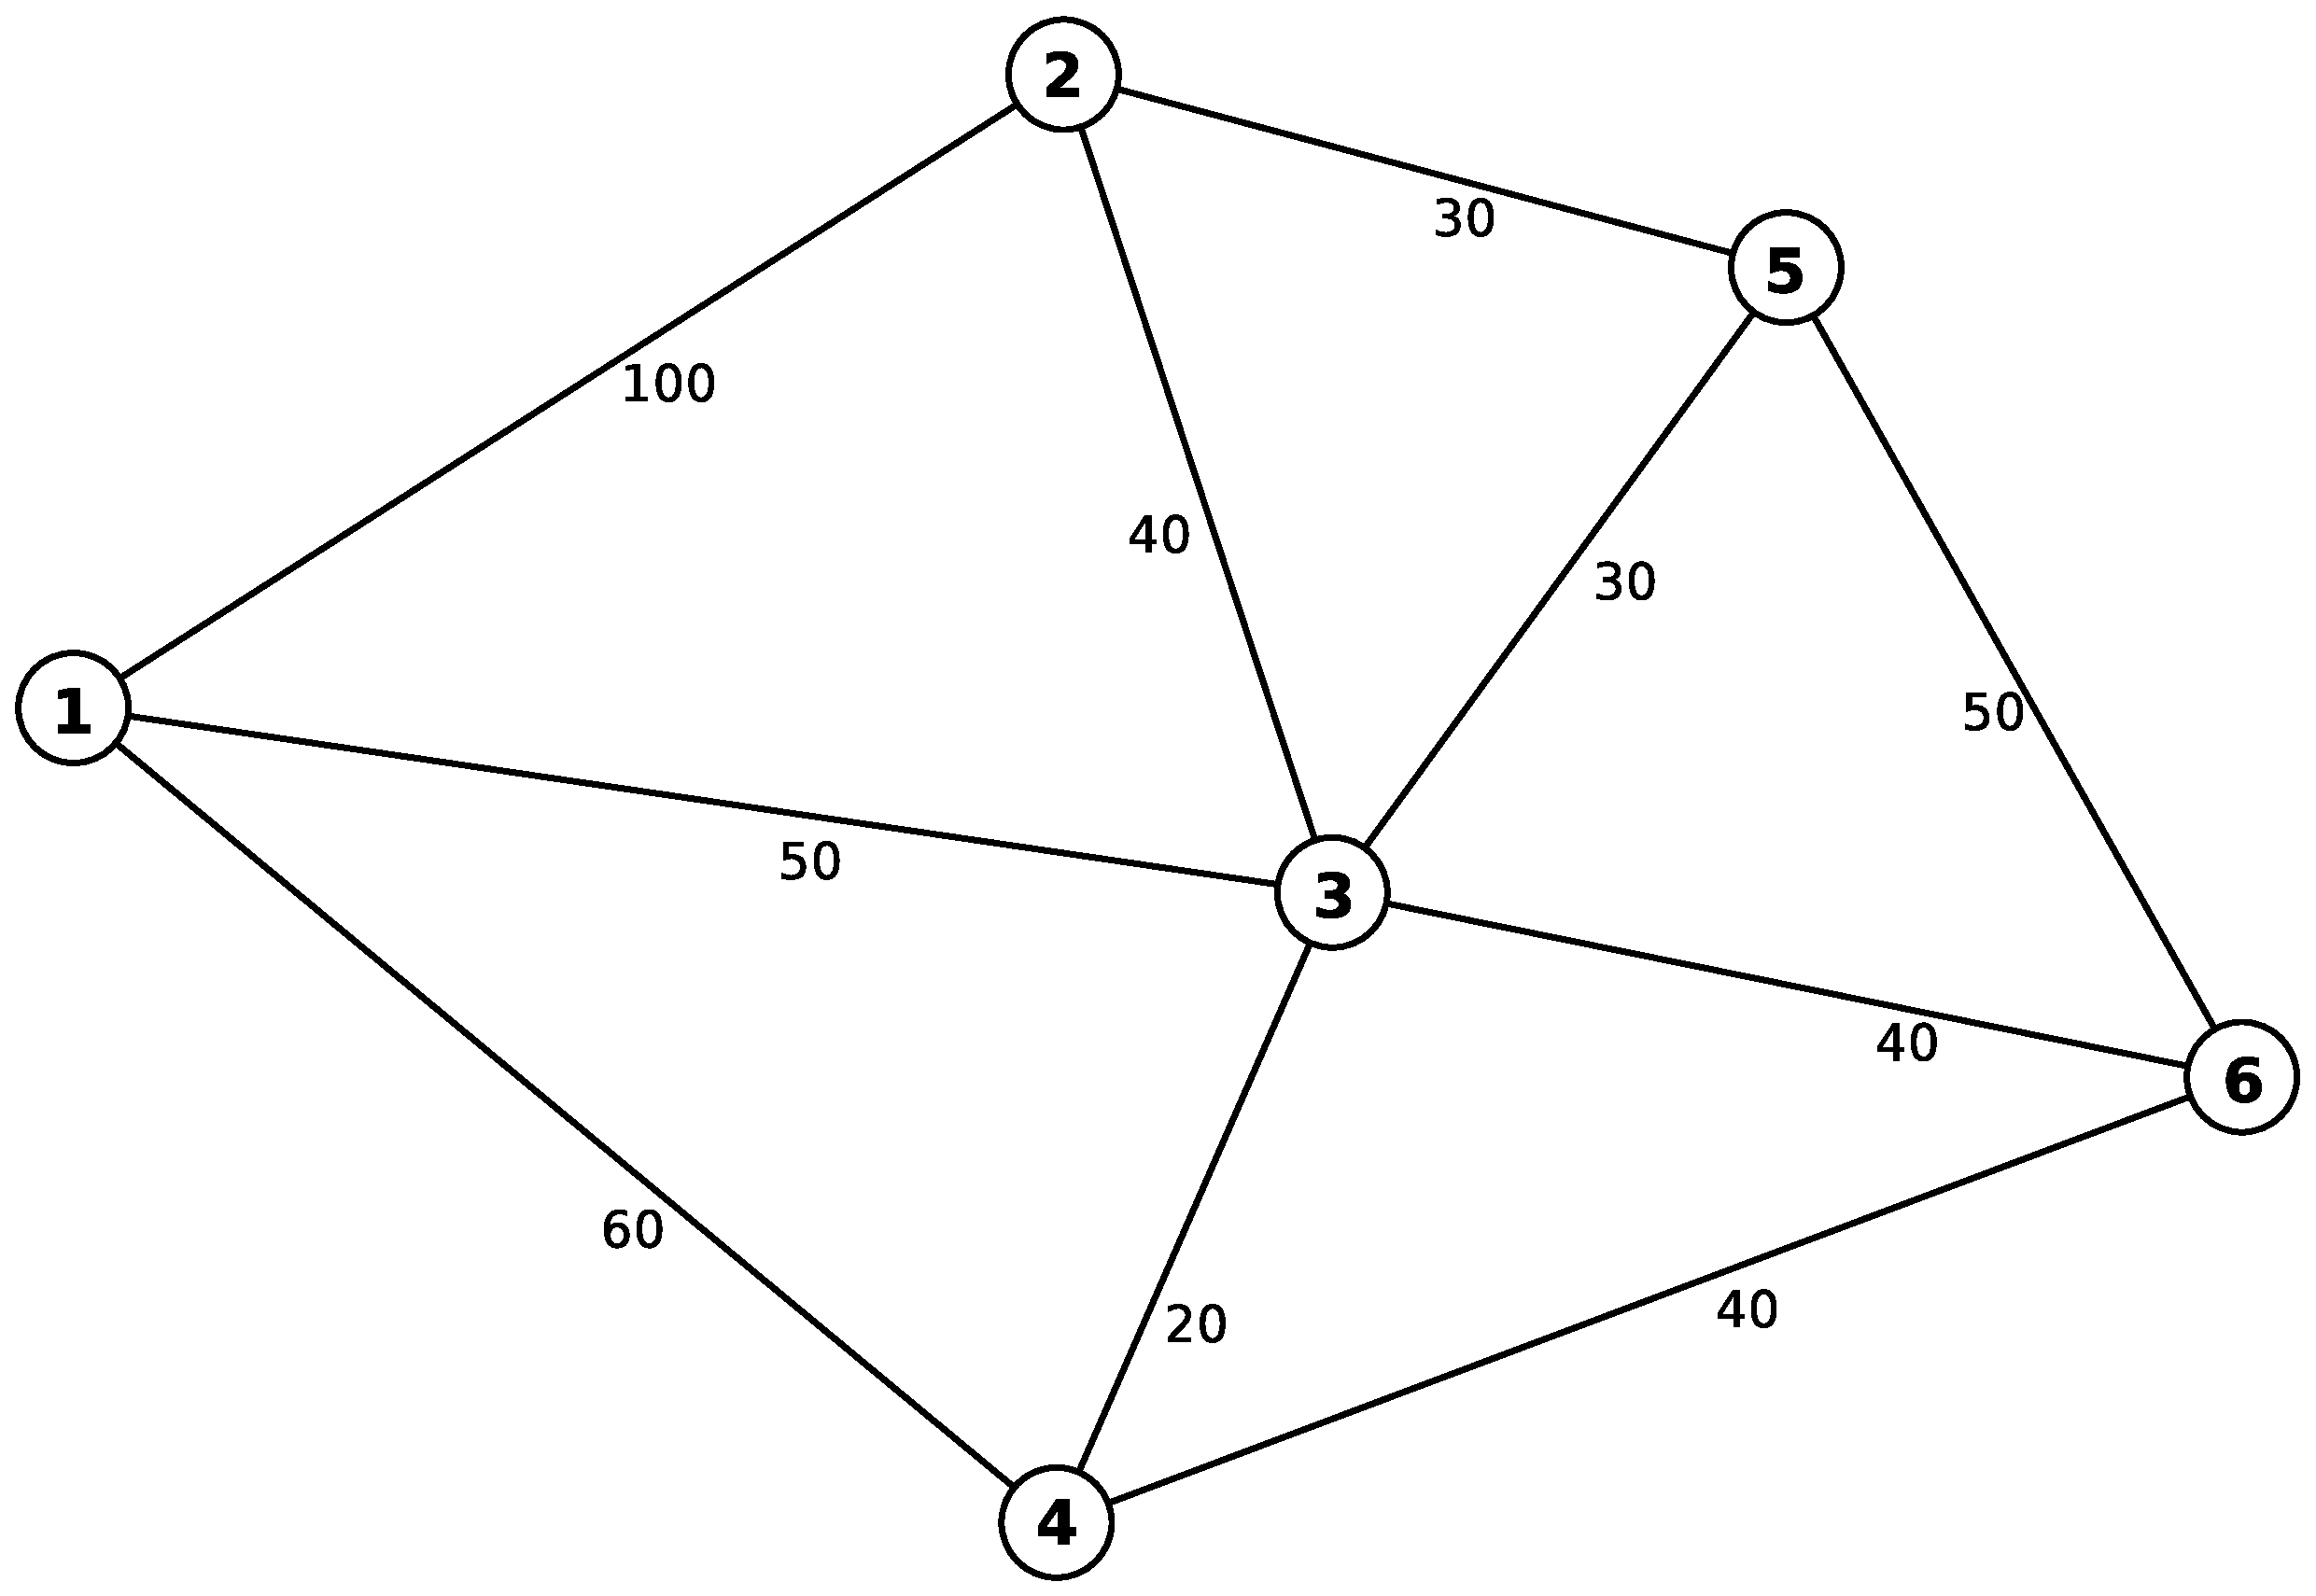
\includegraphics[scale=0.1]{images/figura.eps}
\begin{figure} [h]
\begin {center}
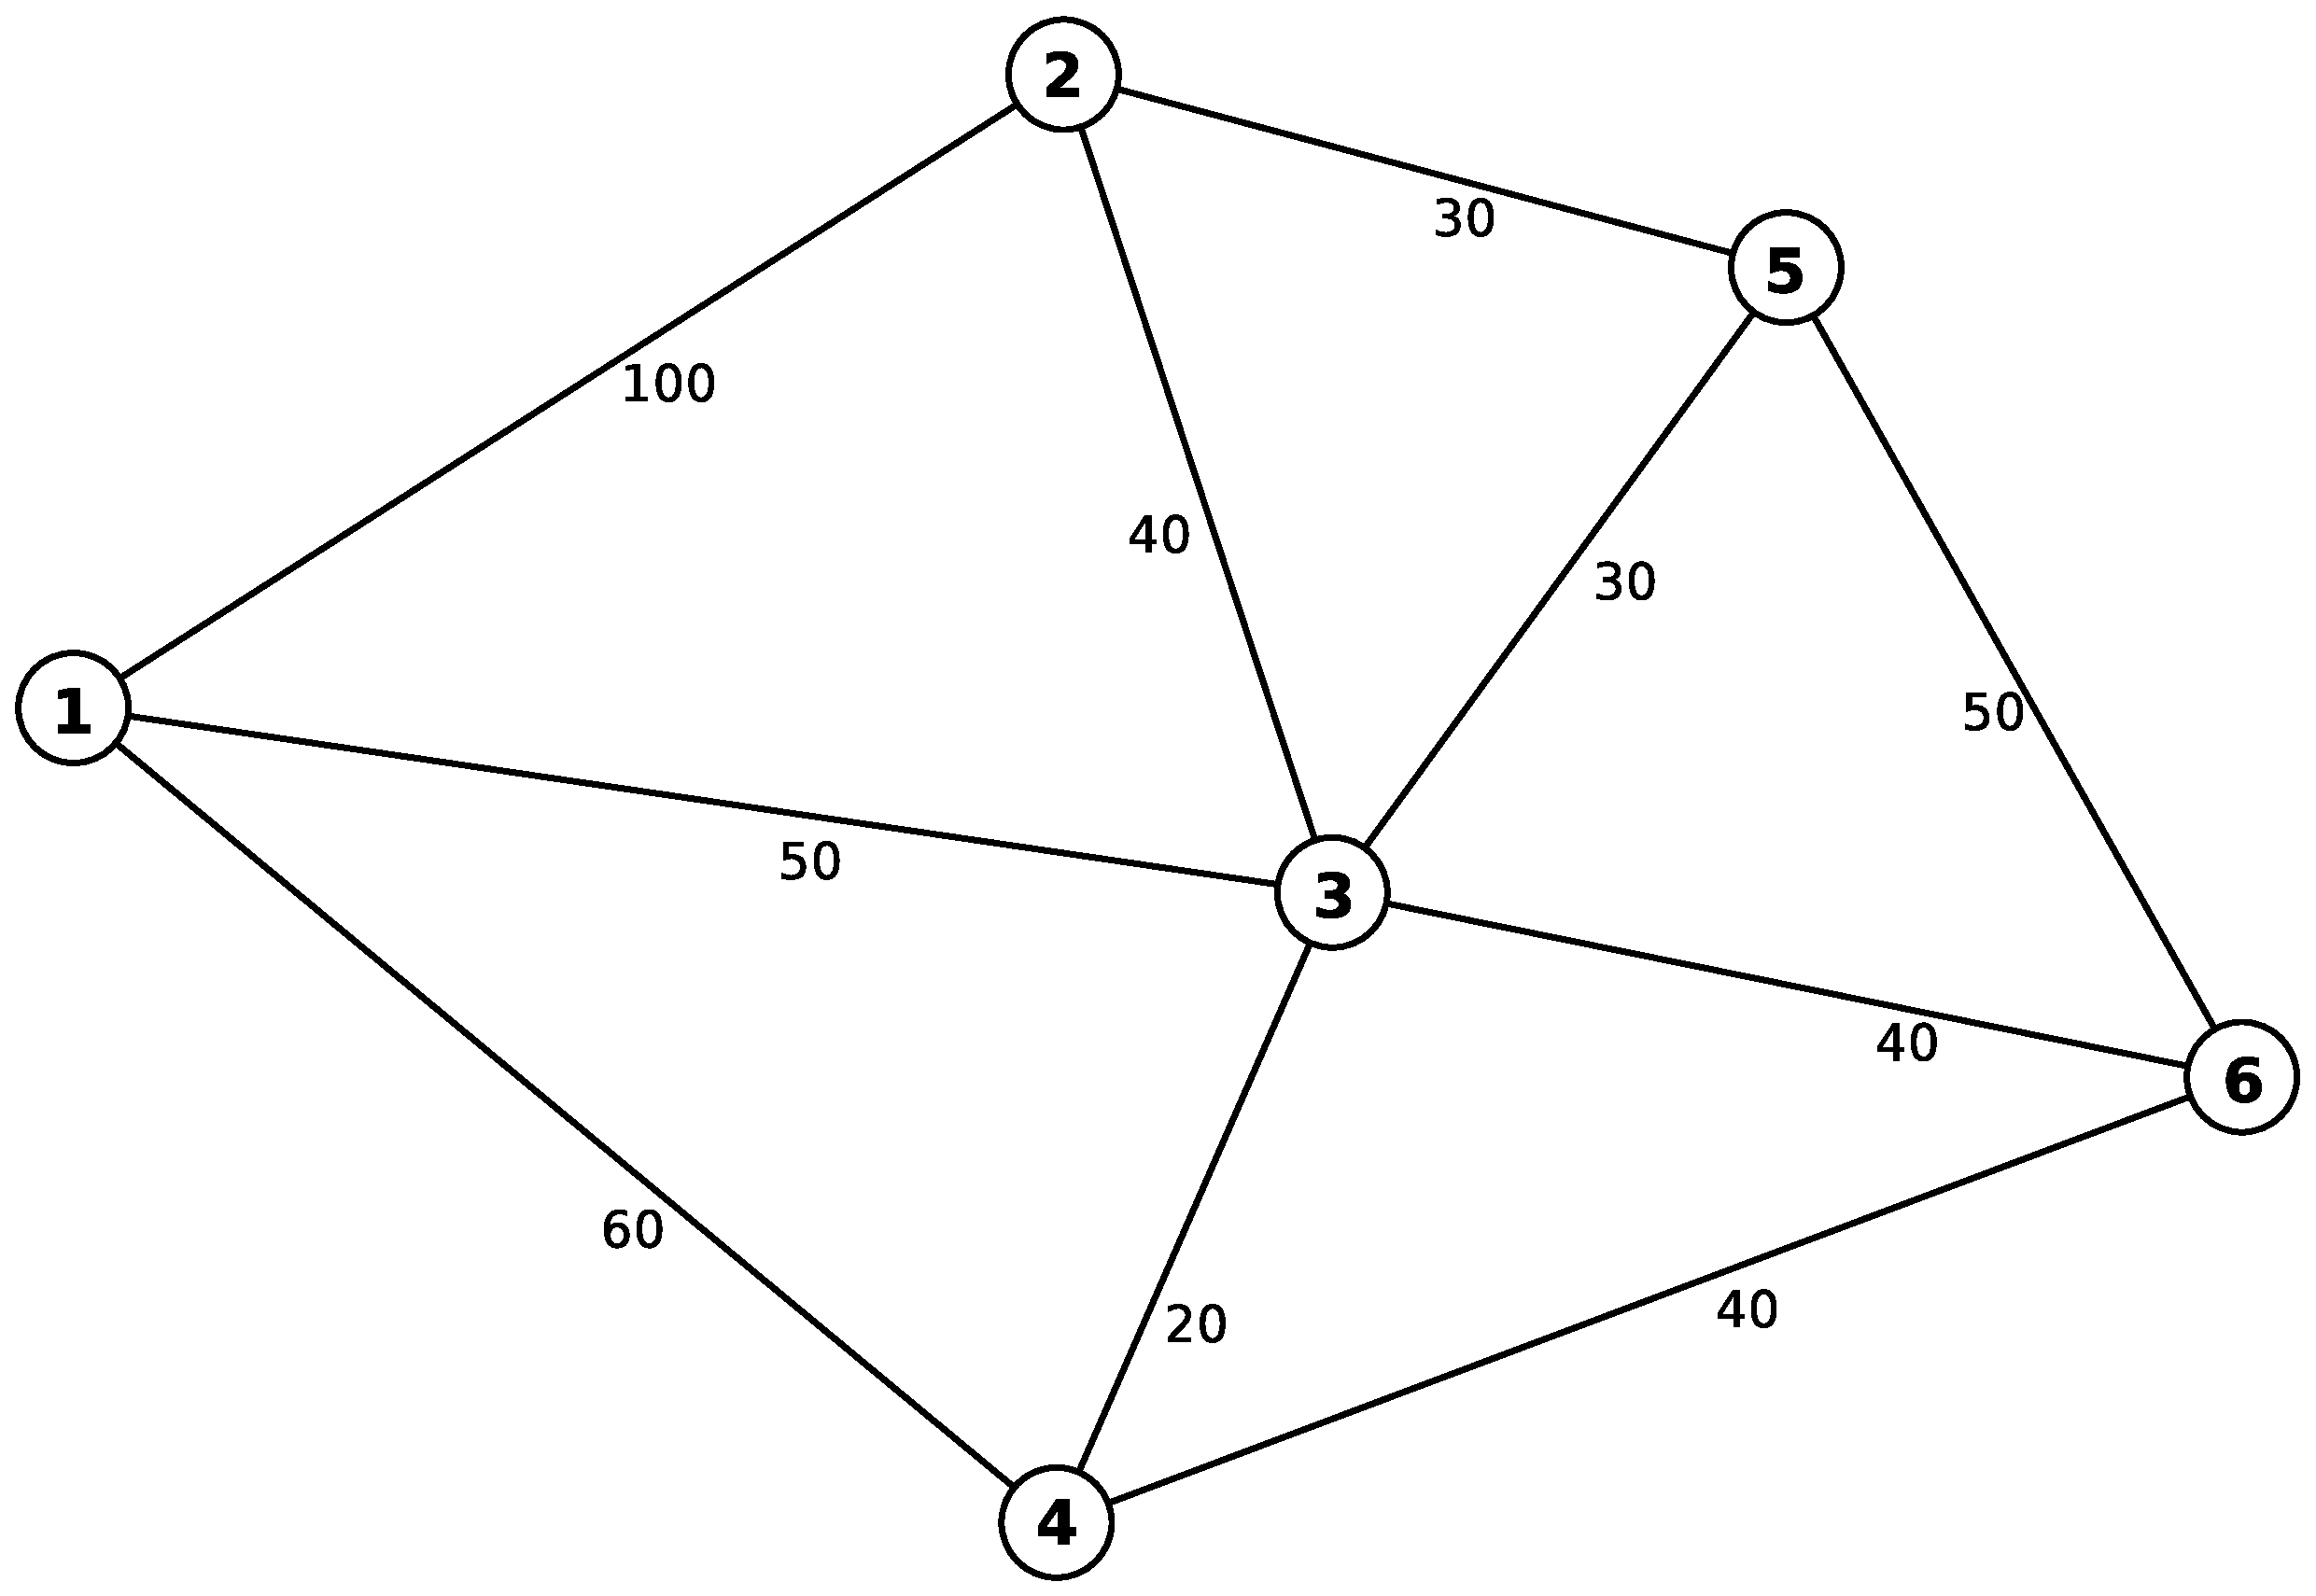
\includegraphics[width=0.8\textwidth]{images/figura.eps}
\end {center}
\end{figure}


En los arcos se definen las capacidades que cada uno de estos puede mantener circulando, en
metros cúbicos por hora.\\

Usando los métodos conocidos responda:\\

1. Determine el flujo máximo que puede entregarse a los generadores. Realice los cálculos de 
\hspace*{0.9cm}forma iterativa y en cada una especifique el flujo acumulado.\\

2. Formule un modelo de programación lineal que le permita satisfacer las restricciones y obtener 
\hspace*{0.9cm}el flujo máximo.\\

3. Realice el mismo trabajo, usando software LINDO o LPSolve. Adjunte sus códigos y comente
\hspace*{0.9cm}sus resultados.\\
